\documentclass[a4paper 
%,11pt 
,twoside
]{article}


\usepackage[utf8]{inputenc}
\usepackage{geometry}
\setlength{\headheight}{13.6pt}
\geometry{left=33.02mm, right=33.02mm, bottom=25mm}
\usepackage{tabularx}
\usepackage{imakeidx}
\usepackage{color}   %To colour the links
\usepackage[dvipsnames]{xcolor}
\usepackage{imakeidx}
\usepackage{svg}
\usepackage{amsmath}
\raggedbottom 
\usepackage[
  pdftex,
  pdfauthor={Eduardo Nolla},
  pdftitle={BBDD LSMotor},
  pdfsubject={BBDD},
  pdfproducer={LaTeX},
  pdfcreator={pdfLaTeX},
  pdfduplex={DuplexFlipLongEdge}, %Alt.: Simplex or DuplexFlipShortEdge 
  pdflang={es}, % en
%  bookmarksopen,
%  bookmarksnumbered,
]{hyperref}
\hypersetup{urlcolor=blue}
\usepackage[spanish]{babel}

\hypersetup{
    colorlinks=true, %set true if you want colored links
    linktoc=all,     %set to all if you want both sections and subsections linked
    linkcolor=Blue,  %choose some color if you want links to stand out
}
\usepackage{fancyhdr}
\usepackage[utf8]{inputenc} % Required for inputting international characters
\usepackage[T1]{fontenc} % Output font encoding for international characters
%\usepackage{fouriernc} % Use the New Century Schoolbook font
\usepackage{graphicx}
\graphicspath{ {D:\OneDrive\Estudios\uni\Curso_2\paed\practicas\proyecto2\latex\imagenes} }
\pagestyle{fancy}
\fancyhf{}
\fancyhead[EL,RO]{Eduardo Nolla}
\fancyhead[ER,LO]{Bases De Datos}
\fancyfoot[ER,LO]{\leftmark}
\fancyfoot[EL,RO]{\thepage}
 
\renewcommand{\headrulewidth}{1pt}
\renewcommand{\footrulewidth}{1pt}




\title{PAED Práctica 3 - CSGO}
\author{Eduardo Nolla}
\date{July 2020}
\usepackage{bookmark}
\usepackage[autostyle=true]{csquotes}

\input{settings/listings.tex}
\input{settings/bibliography.tex}
\input{settings/colors.tex}

%\renewcommand*\contentsname{Índice}
\usepackage{pdfpages}
\usepackage{minted}

\graphicspath{ {images/} }


\definecolor{LightGray}{gray}{0.9}
\definecolor{DarkGray}{RGB}{37, 37, 37}

%\pagecolor{DarkGray}

\usemintedstyle{monokai}

%New colors defined below
\definecolor{codegreen}{rgb}{0,0.6,0}
\definecolor{codegray}{rgb}{0.5,0.5,0.5}
\definecolor{codepurple}{rgb}{0.58,0,0.82}


\begin{document}
\input{resources/title_page.tex}

\newpage\thispagestyle{empty}
{
  \pagestyle{empty}
  \addtocontents{toc}{\protect\thispagestyle{empty}} 
  \tableofcontents
  \clearpage
}

\section{Introduction With a Brief Summary}
  \paragraph{}
  Se debe realizar una importación de la base de datos alojada en Puigpedrós hacia una base de datos local de tipo OLTP.
  \paragraph{}
  Dentro de la tabla OLTP dispondremos de unos triggers que se dedicarán a ir exportando todas las tablas hacia las nuevas tablas mejor optimizadas a nivel de rendimiento llamadas OLAP.
  \paragraph{}
  Entonces tendremos dos tablas locales. La tabla OLTP (optimizada a nivel de almacenamiento) y la tabla OLAP (optimizada a nivel de rendimiento).
  \paragraph{}
  Para hacer la comparativa, se van a realizar distintas queries que nos van a permitir encontrar la verdadera eficacia del uso de este tipo de tablas.

\pagebreak
\section{OLAP and OLTP concepts explained}
  \paragraph{}
  OLTP es un tipo de Base de Datos normalizado según las normas formales. Se centra en la optimización del almacenamiento de las tablas. Mientras que el modelo OLAP se centra más en juntar tablas previsiblemente debamos tener juntas en las futuras queries. 
  \paragraph{}
  Por ejemplo, la tabla de nombres de usuario y la tabla de correos electrónicos es muy probable que en las consultas se tenga que realizar un JOIN entre ellas, teniendo un coste alto. Precisamente en OLAP, al tener esas tablas ya juntas, ahorramos en tiempos de ejecución.


  \subsection{OLAP}

    OLAP, viene de las siglas Online Analytical Processing y su uso más importante, como su nombre indica es el Análisis de información.
    
    \subsubsection{Ventajas de OLAP}
    \begin{itemize}
      \item   OLAP es una plataforma que se incluye en todo tipo de negocios, incluyendo planificación, reportes, anális\dots
      \item Los cálculos y la información son consistentes dentro de OLAP.
      \item Podemos buscar con mucha facilidad términos específicos
      \item Tiene un tiempo de respuesta para el análisis de datos muy veloz.
    \end{itemize}

    \subsubsection{Desventajas de OLAP}
    \begin{itemize}
      \item OLAP requiere un tipo especifico de ordenación de la información como STAR o SNOWFLAKE schema. Son sistemas complicados de implementar y de administrar.
      \item No se pueden tener muchas dimensiones en un solo cubo OLAP
      \item Los datos transaccionales no se pueden acceder dentro de un sistema OLAP
      \item Cualquier modificación en el cubo OLAP, requiere una actualización completa
    \end{itemize}


    \subsubsection{Tipos de OLAP}
    Hay diferentes tipos de Bases de Datos OLAP.
    \begin{enumerate}
      \item ROLAP: Relational OLAP, es el más estándar y eficiente
      \item MOLAP: Implementa las operaciones multidimenionales
      \item HOLAP: Hybrid OLAP. Es una mezcla enre ROLAP y MOLAP
      \item WOLAP: Web OLAP. Es un sistema OLAP accesible desde el navegador
      \item DOLAP: Desktop OLAP. El usuario se descarga una parte de la BBDD en su ordenador y la analiza ahí.
      \item MOLAP: Mobile OLAP. Permite al usuario acceder a través de un dispositivo móvil
      \item SOLAP: Spatial OLAP. Facilita el trabajo en sistemas espaciales de datos como Geographic Information System
    \end{enumerate}

    \subsubsection{ROLAP Advantages}
    Nosotros, vamos a usar el primero de todos en nuestra Base de Datos. Sus mayores ventajas, son que ofrece una alta eficiencia de datos ya que las queries nos salen altamente optimizadas.
    \paragraph{}
    Ofrece también mucha escalabilidad, por si queremos añadir muchos más datos a nuestra base 

    \subsubsection{ROLAP Drawbacks}
    ROLAP necesita una alta utilización de potencia bruta, software y hardware. Ya que usa herramientas SQL, el calculo de los datos agregados es limitado. Y comparandolo con MOLAP, su rendimiento es menor.

  \subsection{OLTP}
  OLTP puede ser usada para las transacciones diarias de una organización. Básicamente se centra en el procesamiento analítico de consultas, como sus siglas indican (Online Transaction Processing).

  \paragraph{}
  Tiene diferentes características, entre las que destacan:
  \begin{itemize}
    \item Transacciones con cantidades pequeñas de datos.
    \item Acceso fácil a esos datos
    \item Gran cantidad de usuarios
    \item Tiempo de respuesta veloz
    \item Esquema Normalizado según las formas normales
    \item Menor uso de espacio de disco.
  \end{itemize}

  \paragraph{}
  Los sistemas de datos OLTP están más ambientados a la transacciones. Lo que significa que al analizar este tipo de situaciones, se van a comportar con mejor rendimiento. Veamos un ejemplo de cuando nos puede ser útil OLTP:

  \paragraph{}
  Supongamos que varias personas están intentando comprar al mismo tiempo las entradas de un partido de fútbol. Cada persona va a escoger un asiento y va a comprar una entrada a distinto precio.

  \paragraph{}
  Entonces, debemos asegurarnos de que dos personas distintas, no compren la misma entrada o que de las personas que están comprando más tarde no compren entradas que no existen. 

  \paragraph{}
  Es en este caso, que podemos ver como las transacciones son mucho más eficaces en una Base de Datos OLTP que nos ayude a manejar este tipo de situaciones.



  \subsection{Ventajas OLTP}
  \begin{itemize}
    \item Tareas de inserción, actualización y eliminación.
    \item Consistencia y concurrencia
    \item Bueno para operaciones perqueñas
  \end{itemize}
  \subsection{Desventajas OLTP}
  \begin{itemize}
    \item Más insegura frente a delincuentes
    \item Número limitado de consultas
    \item Si hay fallos se pueden perder grandes cantidades de datos
    \item Más personal trabajando
  \end{itemize}

  \subsection{Diferences between them}

  \begin{table}[htbp]
    \begin{center}
    \begin{tabular}{|l|l|}
    \hline
    OLTP & OLAP \\
    \hline \hline
    Gran cantidad de transacciones cortas & Gran volumen de datos \\ \hline
    Sistema de Modificación de BBDD & Sistema de gestión de BBDD \\ \hline
    Insert, Update, Delete & Select \\ \hline
   Datos provienen de  & OLTP como fuente de datos \\ \hline
    Orientado a mercado & Orientado a Cliente \\ \hline
    Consultas sencillas & Consultas complejas, agregaciones \\ \hline
    Orientado a aplicación & Orientado a temas \\ \hline
    Operaciones en tiempo real & Análisis por categoria y atributos \\ \hline
    \end{tabular}
    \caption{Tabla comparativa.}
    \label{tabla:sencilla}
    \end{center}
    \end{table}

\pagebreak
\section{Explain How You Find Out The Remote OLTP Database Structure}

  \paragraph{}
  Para encontrar la estructura de la base de datos remota, se ha conectado al servidor de Puigpedros y desde ahí a la base de datos. 

  \paragraph{}
  Desde la línea de comandos se ha usado el comando Show Databases para ver las bases de datos a las que tenemos acceso.

  \paragraph{}
  Ejecutamos el use F1; para usar la base de datos F1 y recibimos el resultado de: Figura \ref{tablas}

  \begin{figure}[H]
    \centering
    \label{tablas}
    \includegraphics[width=8cm]{tables.png}  
    \caption{Todas las Tablas de la Base de Datos}

  \end{figure}


  \paragraph{}
  Ejecutamos Show tables; para ver todas las tablas que hay en F1

  \paragraph{}
  Luego vamos ejecutando de manera individual los describe en la Figura \ref{table_columns}

  \begin{figure}[H]
    \centering
    \label{table_columns}
    \includegraphics[width=8cm]{table_columns.png}
    \caption{Columnas en la tabla circuits}
  \end{figure}

\pagebreak
\section{Relational OLAP Model Diagram}
\includepdf[]{resources/bbdd_p2.pdf}
\pagebreak
\section{Explain How Your Java Program Works}
  \paragraph{}
  Este programa usa una librería:\\
  -	OpenCSV\\
  Se descarga de manera automática desde Maven 
  \paragraph{}
  En primer lugar, nos conectamos a la base de datos remota, con ayuda de la librería JDBC de MySQL. Luego realizaremos un bucle que nos haga un select de las distintas tablas. El resultado lo introduciremos dentro de un ResultSet. Este result set lo exportaremos como CSV gracias a nuestra segunda librería OpenCSV. Por último, importaremos el CSV desde la base de datos OLTP local haciendo uso de LOAD DATA. Después vamos a repetir el proceso con la siguiente tabla.
  \paragraph{}
  Este método se ha usado ya que es mucho menos costo de implementar, ya que no pasa por las clases de Java. Así que nos ahorramos la extracción del ResulSet a su Clase. Y el único coste es el de tener generado el CSV.

  \paragraph{}
  Las clases utilizadas se pueden encontrar en la documentación del proyecto.
  \pagebreak
\section{Explain How You Created The Users}
  \begin{figure}[H]
    \centering
    \includegraphics[width=8cm]{privilege.png}
    \caption{Tipos de privilegios}
  \end{figure}
  \paragraph{}
  Para la creación de usuarios, lo primero que se hace es una comprobación de que no exitan esos mismos usuarios ya en nuestra Base de Datos.

  \paragraph{}
  Posteriormente, vamos a crear los tres usuarios para que puedan acceder a nuestra base de datos localhost.

  \paragraph{}
  Finalmente, vamos a dar permisos de SELECT, CREATE VIEW, SHOW VIEW para la base de datos olap a nuestro analytic user.\\ Vamos a dar permisos de SELECT, INSERT, UPDAATE, USAGE, DELETE  a nuestro usuario manager para la base de datos f1.\\Vamos a dar permisos de creación se usuarios a nuestro usuario de RRHH.



  \begin{listing}[H]
    \begin{minted}[bgcolor = DarkGray, breaklines = true, fontsize=\footnotesize]{SQL}

      USE f1;


    DROP USER IF EXISTS analytic_userm;
    DROP USER IF EXISTS manage_user;
    DROP USER IF EXISTS rrhh_user;

    CREATE USER 'analytic_user'@'localhost', 'manager_user'@'localhost', 'rrhh_user'@'localhost';

    GRANT SELECT, CREATE VIEW, SHOW VIEW ON f1_olap.* to 'analytic_user'@'localhost';

    GRANT SELECT, INSERT, UPDATE, USAGE, DELETE ON f1.* to 'manager_user'@'localhost';  

    GRANT CREATE USER ON *.* TO 'rrhh_user'@'localhost';

    \end{minted}
    \caption{User Creation}
    \label{lst:users}
  \end{listing}

\pagebreak
\section{Explain How Your Stored Procedures Work}
\pagebreak
\section{Explain How Your Events And Triggers Works}
  \subsection{Triggers}
    \paragraph{}
    Después de una inserción dentro de alguno de los campos de la base de datos OLTP se va a actualizar los campos correspondientes dentro de la tabla OLAP, el problema viene cuando en la OLAP hemos juntado distintas tablas en una sola.
    \paragraph{}
    La solución ha sido buscar si el campo que se ha insertado en la OLTP ya existe en la OLAP. Si ya existe lo que vamos a hacer es una actualización mientras que si no existe, vamos a realizar una inserción.

    \begin{listing}[H]
      \begin{minted}[bgcolor = DarkGray, breaklines = true, fontsize=\footnotesize]{SQL}
          IF EXISTS(SELECT * FROM f1_olap.circuits c WHERE c.circuitId = NEW.circuitId) THEN

          update f1_olap.circuits
          SET circuitId  = NEW.circuitId,
              circuitRef = NEW.circuitRef,
              name       = NEW.name,
              location   = NEW.location,
              country    = NEW.country,
              lat        = NEW.lat,
              lng        = NEW.lng,
              alt        = NEW.alt,
              url        = NEW.url
          WHERE circuitId = NEW.circuitId;



        ELSE

          insert into f1_olap.circuits (circuitId, circuitRef, name, location, country, lat, lng, alt, url)
          select NEW.circuitId,
                NEW.circuitRef,
                NEW.name,
                NEW.location,
                NEW.country,
                NEW.lat,
                NEW.lng,
                NEW.alt,
                NEW.url;

        END IF;

      \end{minted}
      \caption{Insertion}
      \label{lst:insert}
    \end{listing}

  \subsection{Events}
\pagebreak
\section{Report about OLTP vs OLAP Comparison}
  \begin{figure}[H]
    \centering
    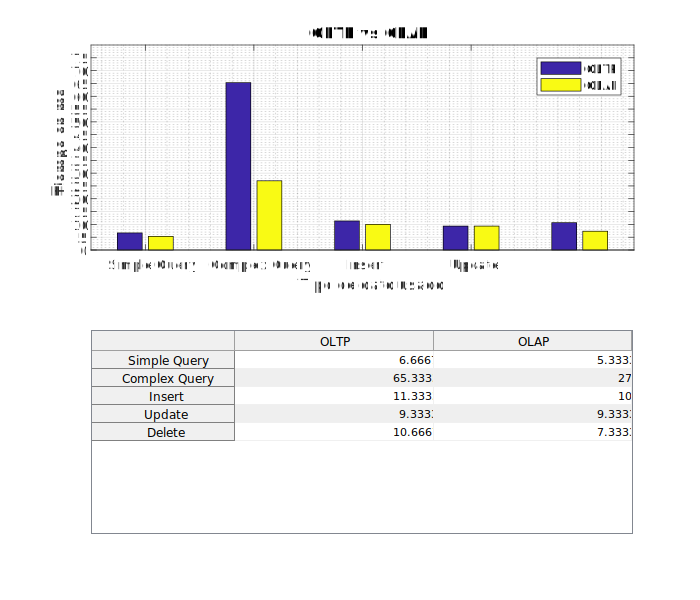
\includegraphics[width=0.8\textwidth]{graficas.png}
    \caption{Gráficas tiempo}
    \label{fig:specular}
  \end{figure}

\paragraph{}
El caso donde podemos ver con mayor claridad la diferencia de uso entre OLTP y OLAP es, principalemente en las queries complejas. Mientras que, como se haa visto antes, en el resto de operaciones. Ambas son muy optimas o inculo es un poco mejor usar OLTP.

\paragraph{}
Anque con los datos actuales, podríamos decir que tardan lo mismo.

\paragraph{}
En el caso de que trabajasemos con mayores volúmenes de datos durante la inserción y la eliminación, podríamos ver con más claridad estas diferencias.

\paragraph{}
De hecho, se puede ver con más claridad, al realizar las inserciones iniciales. La base de datos OLTP es mucho más eficaz al hacer las inserciones que la OLAP. Tardando la primera cerca de 1 minuto mientras que la seguna tarda varias horas.
\pagebreak
\section{Time Dedicated Per Part}
\pagebreak
\section{Conclusiones}
Podemos conluir, que de cara a realizar consultas complejas y al trabajar con largos volúmenes de datos en operaciones que requieren procesamiento intenso, acabamos viendo como es más eficaz usar una Base De Datos de tipo OLAP. Que al final no deja de ser una OLTP desnormalizada.

\paragraph{}
Mientras que por otro lado, la OLTP es mucho mejor para volúmenes de datos pequeños o para múltiples consultas sencillas.

\pagebreak
  
  \addcontentsline{toc}{section}{Bibliografía}
  \nocite{*}
  \printbibliography[title={Bibliografía}]

\end{document}